
\chapter{项目分析及开发过程}

\section{项目分析}
\subsection{项目一: JDBC}
\textbf{elm\_admin 是饿了么 JDBC 版项目,采用了 JDBC+MySQL 开发,是纯后端的字符界面操作数据库的命令行应用程序。}

\subsubsection{项目技术架构}
- JDK 1.8

- JDBC

- MySQL 数据库

\subsubsection{开发工具}
- STS(spring-tool-suite)

- mysql-5.5.62-winx64

- Navicat Premium 8

\subsubsection{安装部署指南}
\begin{itemize}
  \item 安装 jdk、STS、MySQL
  \item 在 MySQL 数据库中创建数据库 \texttt{elm\_admin},使用数据库脚本 \texttt{elm\_admin.sql} 创建数据库和初始数据。  \item 在 STS 中导入 JavaSE 项目。
  \item 打开 \texttt{com/neusoft/elm/util/DBUtil} 修改数据库密码
  \item 本项目有两个入口:管理员入口、商家入口。
      \begin{itemize}
          \item 运行 \texttt{ElmAdminEntry} 中的 main 函数为管理员入口。
          \item 运行 \texttt{ElmBusinessEntry} 中的 main 函数为商家入口。
      \end{itemize}
\end{itemize}
\subsubsection{整体要求}
1. 项目技术架构

   - JDK8
   
   - JDBC
   
   - MySql
   
2. 开发工具

   - STS(SpringToolSuite4)
   
   - mysql-5.5.62-winx64
   
   - navicat
   
3. 涉及的技术点

   - 封装 JDBC

   - 封装 DAO

   - 领域模型中的实体类
   
   - 增删改查操作

   - 多条件模糊查询

   - JDBC 事务管理
   
   - 表的主外键关系
   

   
\subsection{项目二: Vue3}
\textbf{饿了么前端版项目是采用 HTML、CSS、JavaScript 开发的前端静态网页项目。}

\subsubsection{项目前端技术架构}
- HTML

- CSS

- JavaScript


\subsubsection{开发工具}
- HBuilder

- Chrome 浏览器


\subsubsection{安装部署指南}
- 安装 HBuilder、Chrome

- 将工程导入到 HBuilder 中

- 在 Chrome 浏览器中运行 index.html 文件

- 在 Chrome 浏览器中使用 Toggle device toolbar 模拟手机浏览

\subsubsection{整体要求}
1. 项目技术架构

   - HTML5

   - CSS3

   - JavaScript(ES6 以上)

   
2. 开发工具

   - HBuilder

   - Chrome 浏览器

   
3. 涉及的技术点

   - HTML5 标签的使用

   - CSS3 样式的使用

   - JS 对 DOM 的基本操作

   - DIV+CSS 布局基础

   - 移动端布局基础

   - viewport 设置

   - 弹性布局

   - 边框盒子模型

   - vw 与 vh 的使用

   - 图片按比例自适应

   - CSS3 小图标的使用

   - 第三方字体库的使用



\subsection{项目三: Servlet}

% 仅添加换行
\textbf{饿了么 Servlet 版本}

\subsubsection{项目演示}
- 运行 “饿了么项目”,演示应用程序效果,演示 “点餐业务线” 整体流程。

- 本项目参照 “饿了么官网网页版” 制作。饿了么网页版:http://h5.ele.me/

- 本项目专注于完成点餐业务线功能,“饿了么官网” 中的其它功能暂不涉及。


\subsubsection{项目目标}
- 本项目为课程级贯穿项目中的第三个项目(JDBC项目、前端项目、JavaWeb项目)。

- 本项目完成后,学员将能够使用 Vue + Servlet + AJAX 技术开发前后端分离的 Web 应用程序。

\subsubsection{项目中所涉及到相关知识点}
- AJAX 的使用

- Servlet 的使用

- Session 的使用

- 简单 MVC 封装

- Service 层事务管理

- DAO 层批量操作

- 多对一与一对多的映射

- 服务器端 JSON 数据转换

- VueCLI 的使用

- 多条件模糊查询的使用

- SVN、Git 版本控制工具的使用

\subsubsection{数据库设计}
- 本项目完成后,学员将能够使用 Vue + Servlet + AJAX 技术开发前后端分离的 Web 应用程序。

\subsubsection{整体要求}
1. 项目技术架构

- JDK8

- Servlet

- Tomcat5.5

- MySQL

- Vue
   
2. 开发工具

- HBuilder

- STS(SpringToolSuite4)

- mysql-5.5.62-winx64

- Tomcat8.5
   
3. 涉及的技术点

- AJAX 的使用

- Servlet 的使用

- Session 的使用

- 简单 MVC 封装

   - Service 层事务管理

   - DAO 层批量操作

   - 多对一与一对多的映射

   - 服务器端 JSON 数据转换

   - VueCLI 的使用

   - 多条件模糊查询的使用


\subsection{项目四: SpringBoot}
\textbf{饿了么 SpringBoot 版本}

\subsubsection{整体要求}
1. 项目技术架构

- JDK8

- SpringBoot

- MyBatis

- MySQL

- Vue



2. 开发工具

- HBuilder

- STS(SpringToolSuite4)

- mysql-5.5.62-winx64

- Tomcat8.5

- Maven



3. 涉及的技术点

- AJAX 的使用

- SpringBoot 框架的使用

- MyBatis 框架的使用

- 封装 Mapper

- Service 层事务管理

- 数据层批量操作

- 多对一与一对多的映射

- 服务器端 JSON 数据转换

- VueCLI 的使用

- 多条件模糊查询的使用

\section{开发过程}

\begin{itemize}
    \item \textbf{项目进度:}
    \begin{itemize}
        \item 第一周:学习了项目一的内容,复盘了项目一的代码;
        \item 第二周:学习了项目二到项目四的内容,复盘了项目二到项目四的代码,饿了吧V1.0项目复盘完成,并完成了前后端的部署;
        \item 第三周:创新了原项目,饿了吧V2.0项目完成,前后端数据库都部署在了腾讯云服务器上,并制作了简易的手机apk
    \end{itemize}
\end{itemize}

\section{gitee上团队成员贡献}

\begin{figure}[htbp]
    \centering
    \begin{minipage}{0.4\textwidth}
    \centering
    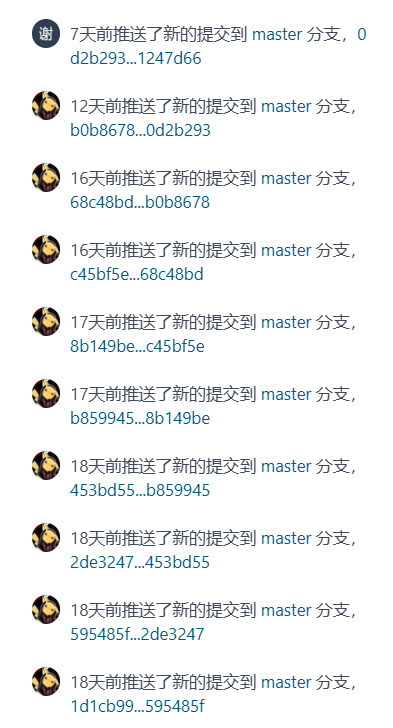
\includegraphics[width=\textwidth]{Picture1}
    \caption{Gitee提交数据1}\label{fig:dd}
    \end{minipage}
    \begin{minipage}{0.4\textwidth}
    \centering
    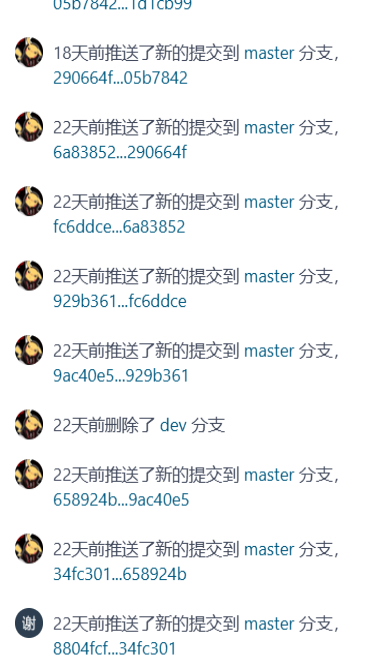
\includegraphics[width=\textwidth]{Picture2}
    \caption{Gitee提交数据2}\label{fig:ds}
    \end{minipage}
    \vspace{\baselineskip}
    \end{figure}

    \begin{figure}[htbp]
        \centering
        \begin{minipage}{0.4\textwidth}
        \centering
        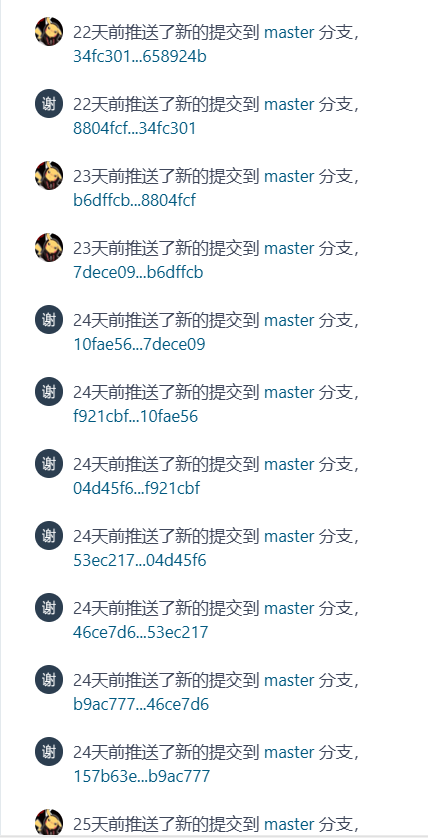
\includegraphics[width=\textwidth]{Picture3}
        \caption{Gitee提交数据3}\label{fig:dd}
        \end{minipage}
        \begin{minipage}{0.4\textwidth}
        \centering
        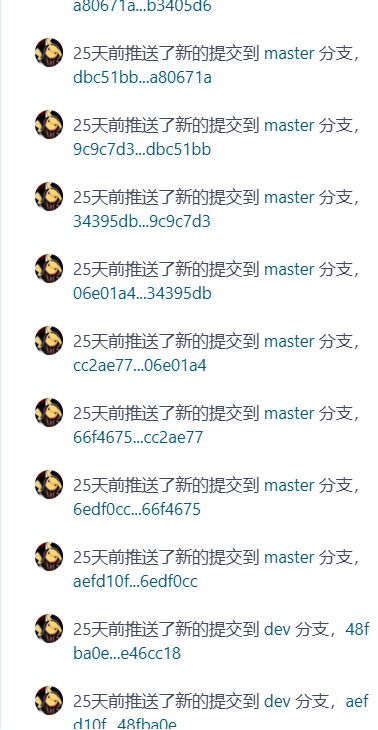
\includegraphics[width=\textwidth]{Picture4}
        \caption{Gitee提交数据4}\label{fig:ds}
        \end{minipage}
        \vspace{\baselineskip}
        \end{figure}
